\begin{figure}
    	\centering
    	\begin{minipage}{0.45\textwidth}
    		\centering

		\textbf{\large \textcolor{color3}{3}\textcolor{color2}{2}\textcolor{color3}{3}\textcolor{color3}{3}\textcolor{color1}{1}\textcolor{color2}{2}\textcolor{color3}{3}\textcolor{color1}{1}\textcolor{color3}{3}}
    		
    		(a)
		\vspace{10mm}  		
    		
    		\textbf{\large \textcolor{color3}{1}\textcolor{color2}{01}\textcolor{color3}{1}\textcolor{color3}{1}\textcolor{color1}{00}\textcolor{color2}{01}\textcolor{color3}{1}\textcolor{color1}{00}\textcolor{color3}{1}}
    		
    		(b)
    	\end{minipage}
    	\begin{minipage}{0.45\textwidth}
    		\centering
    		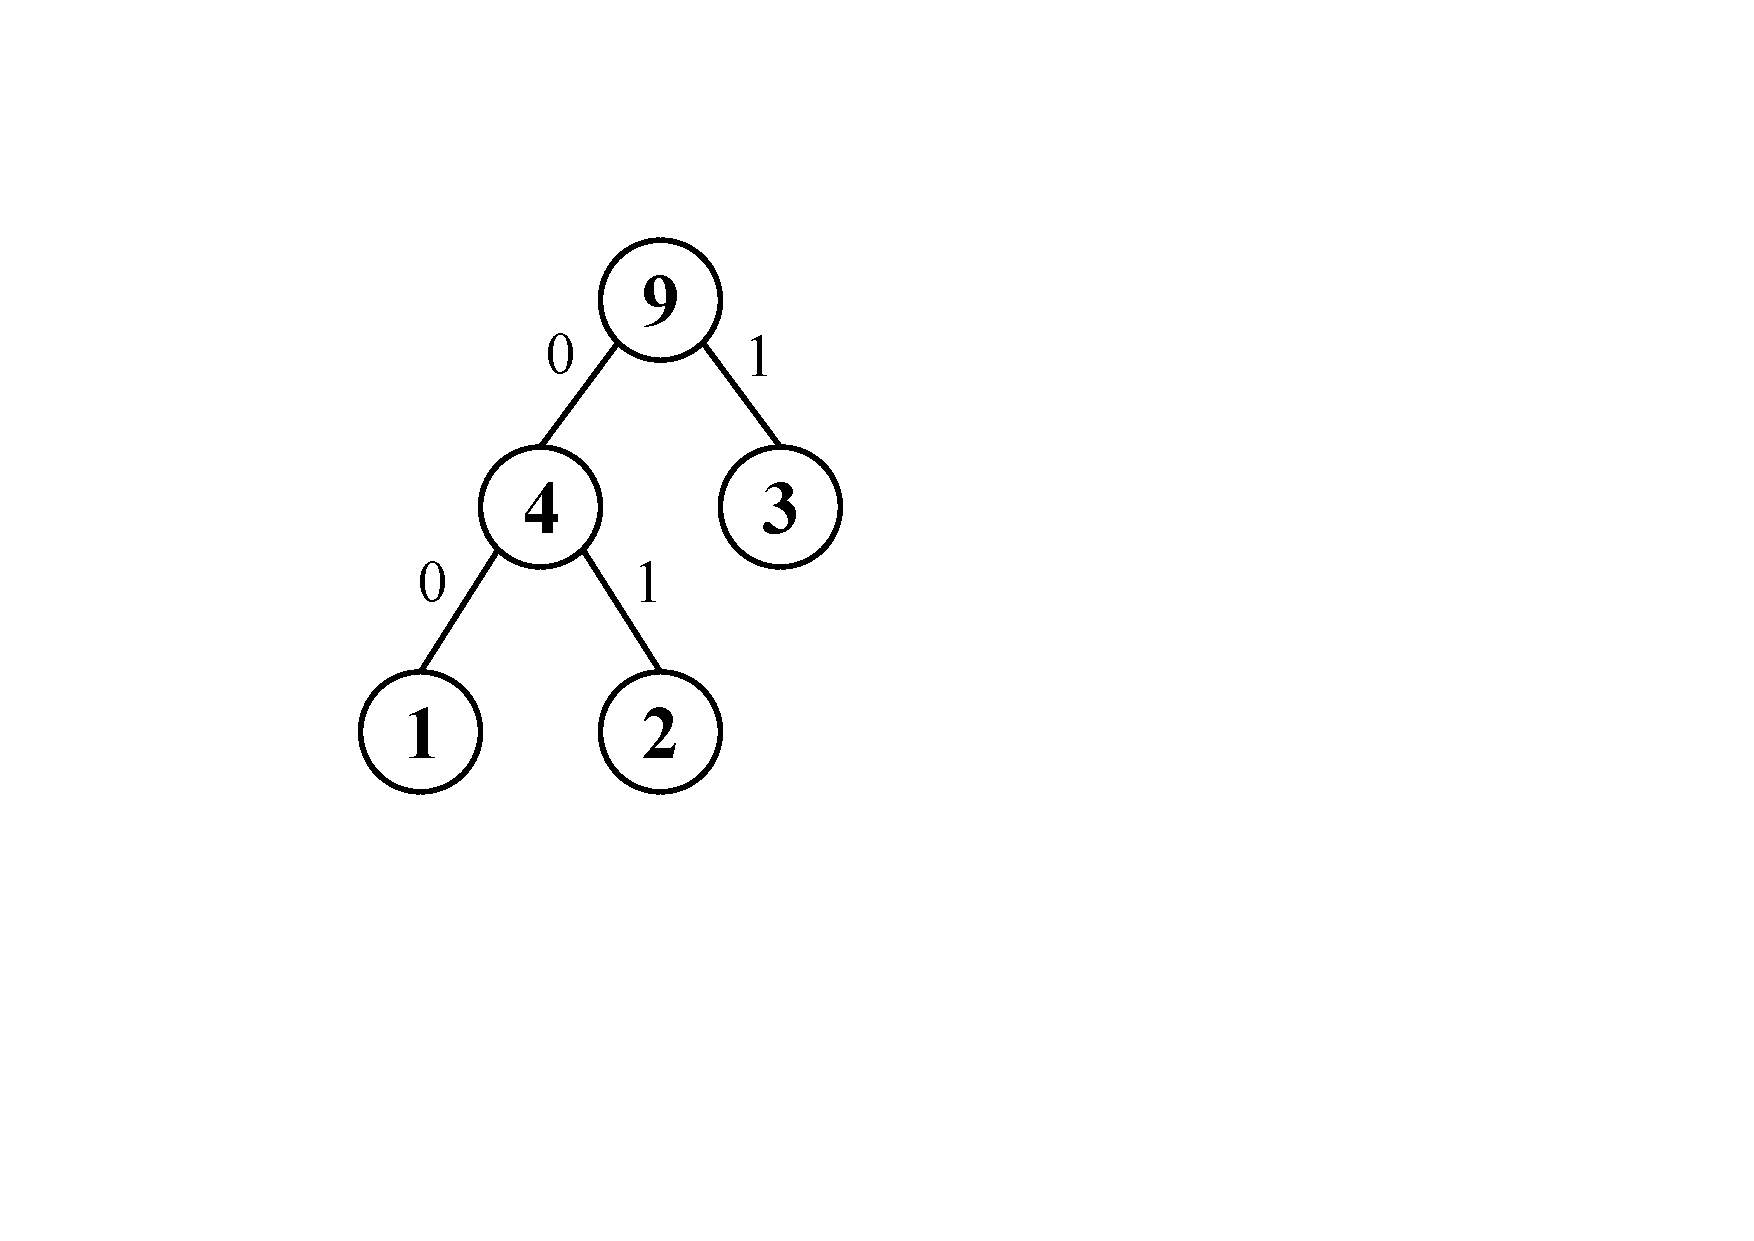
\includegraphics[scale=.4, clip, trim=160 180 410 0]{img/graphs-huffman.pdf}
    		
    		(c)
    	\end{minipage}

    \caption{Ejemplo de codificación Huffman. (a) Secuencia de entrada. (b) Secuencia de salida. (c) Diagrama de vocabulario en árbol binario.}
    \label{fig:huffman}
\end{figure}
